% =============================================================================
% COPYRIGHT AND DISCLAIMER
% =============================================================================
% This file is provided as a convenience template for competition participants.
% By using it, you accept full responsibility for compliance with all applicable
% copyright, licensing, and usage rules of the Association for Computing
% Machinery (ACM) and of any LaTeX packages you load (including, without
% limitation, the "acmart" document class and related ACM materials).
%
% Consult ACM's official publication, template, and copyright policies before
% using this setup for any purpose other than this competition. Do not assume
% that this template may be reused, redistributed, or submitted elsewhere
% without independently verifying ACM's current rules.
%
% Use of the "acmart" class, the "sigconf" option, or ACM-style formatting in
% this template does NOT mean that this report, this competition, its organizers,
% or any resulting PDF is sponsored, endorsed, affiliated with, or published by
% ACM. ACM trademarks and branding remain the property of ACM.
%
% Template packages live in preamble.tex.
% Citations live in main.bib. Edit this file with your paper content.
% =============================================================================
% Figures are read from figures/ (a copy of the used files from ../docs/figures). On Overleaf, upload
% main.tex, preamble.tex, main.bib and the figures/ folder. Local build: tectonic -X compile main.tex

\documentclass[sigconf]{acmart}
% =============================================================================
% Template setup — participants normally do not edit this file.
% Author content belongs in main.tex; citations belong in main.bib.
% \documentclass lives in main.tex so Overleaf does not treat this file as root.
% =============================================================================

% --- Competition / non-ACM-submission friendly rights metadata -------------
\setcopyright{none}
\settopmatter{printacmref=false}
\acmConference[Kaggle Competition]{Filament Segmentation Challenge}{2026}{\href{https://www.kaggle.com/competitions/filament-segmentation-2026}{kaggle.com/competitions/filament-segmentation-2026}}
\acmBooktitle{Competition Report}
\acmDOI{}
\acmISBN{}

% --- Author guidance text --------------------------------------------------
% \guide{...} is gray italic while \guideStyletrue; omitted from the PDF if false.
% Flip the switch in main.tex after % =============================================================================
% Template setup — participants normally do not edit this file.
% Author content belongs in main.tex; citations belong in main.bib.
% \documentclass lives in main.tex so Overleaf does not treat this file as root.
% =============================================================================

% --- Competition / non-ACM-submission friendly rights metadata -------------
\setcopyright{none}
\settopmatter{printacmref=false}
\acmConference[Kaggle Competition]{Filament Segmentation Challenge}{2026}{\href{https://www.kaggle.com/competitions/filament-segmentation-2026}{kaggle.com/competitions/filament-segmentation-2026}}
\acmBooktitle{Competition Report}
\acmDOI{}
\acmISBN{}

% --- Author guidance text --------------------------------------------------
% \guide{...} is gray italic while \guideStyletrue; omitted from the PDF if false.
% Flip the switch in main.tex after % =============================================================================
% Template setup — participants normally do not edit this file.
% Author content belongs in main.tex; citations belong in main.bib.
% \documentclass lives in main.tex so Overleaf does not treat this file as root.
% =============================================================================

% --- Competition / non-ACM-submission friendly rights metadata -------------
\setcopyright{none}
\settopmatter{printacmref=false}
\acmConference[Kaggle Competition]{Filament Segmentation Challenge}{2026}{\href{https://www.kaggle.com/competitions/filament-segmentation-2026}{kaggle.com/competitions/filament-segmentation-2026}}
\acmBooktitle{Competition Report}
\acmDOI{}
\acmISBN{}

% --- Author guidance text --------------------------------------------------
% \guide{...} is gray italic while \guideStyletrue; omitted from the PDF if false.
% Flip the switch in main.tex after \input{preamble}.
%
% Do not use \guide{...} for \email{...}.
\usepackage{xcolor}
\newif\ifguideStyle
\guideStyletrue
\newcommand{\guide}[1]{%
  \ifguideStyle
    {\color{gray!65}\itshape #1}%
  \fi
}

% --- Math ------------------------------------------------------------------
% Do NOT load amssymb (or amsfonts): acmart already loads newtxmath, which
% defines the same symbols (e.g. \Bbbk) and causes a conflict on Overleaf.
% amsmath is already provided by acmart; mathtools extends it.
\usepackage{mathtools}

% --- Figures ---------------------------------------------------------------
% graphicx is already loaded by acmart
\usepackage{subcaption}

% --- Tables ----------------------------------------------------------------
% booktabs is already loaded by acmart
\usepackage{tabularx}
\usepackage{multirow}

% --- Bibliography style is set in main.tex (ACM-Reference-Format) ----------
.
%
% Do not use \guide{...} for \email{...}.
\usepackage{xcolor}
\newif\ifguideStyle
\guideStyletrue
\newcommand{\guide}[1]{%
  \ifguideStyle
    {\color{gray!65}\itshape #1}%
  \fi
}

% --- Math ------------------------------------------------------------------
% Do NOT load amssymb (or amsfonts): acmart already loads newtxmath, which
% defines the same symbols (e.g. \Bbbk) and causes a conflict on Overleaf.
% amsmath is already provided by acmart; mathtools extends it.
\usepackage{mathtools}

% --- Figures ---------------------------------------------------------------
% graphicx is already loaded by acmart
\usepackage{subcaption}

% --- Tables ----------------------------------------------------------------
% booktabs is already loaded by acmart
\usepackage{tabularx}
\usepackage{multirow}

% --- Bibliography style is set in main.tex (ACM-Reference-Format) ----------
.
%
% Do not use \guide{...} for \email{...}.
\usepackage{xcolor}
\newif\ifguideStyle
\guideStyletrue
\newcommand{\guide}[1]{%
  \ifguideStyle
    {\color{gray!65}\itshape #1}%
  \fi
}

% --- Math ------------------------------------------------------------------
% Do NOT load amssymb (or amsfonts): acmart already loads newtxmath, which
% defines the same symbols (e.g. \Bbbk) and causes a conflict on Overleaf.
% amsmath is already provided by acmart; mathtools extends it.
\usepackage{mathtools}

% --- Figures ---------------------------------------------------------------
% graphicx is already loaded by acmart
\usepackage{subcaption}

% --- Tables ----------------------------------------------------------------
% booktabs is already loaded by acmart
\usepackage{tabularx}
\usepackage{multirow}

% --- Bibliography style is set in main.tex (ACM-Reference-Format) ----------

\usepackage{tikz}
\usetikzlibrary{arrows.meta,positioning}
\graphicspath{{figures/}{../docs/figures/}}
\setlength{\emergencystretch}{2em}  % lets lines with long monospace names break without overfull boxes

% Guide styling: \guideStyletrue = show gray italic hints; \guideStylefalse = omit them
% \guideStyletrue
\guideStylefalse

\begin{document}

\title{A Consensus-Trained U-Net with a Learned Component Scorer}  % Replace this with your title
\subtitle{A Solution to the Solar Filament Segmentation Challenge 2026} % DO NOT CHANGE


\author{Mukharbek Organokov}
\email{mukharbek.organokov@gmail.com}

\begin{abstract}
    This report describes our solution to the Solar Filament Segmentation Challenge~2026, a Kaggle competition on automatic segmentation of solar filaments in GONG H-$\alpha$ observations. A single U-Net with a ResNet-34 encoder, run at 1536~px, is trained on the consensus of the annotators and averaged over four flipped views. Its connected components are candidates, and a gradient-boosted component scorer, trained on out-of-fold candidates, predicts each candidate's expected contribution to Panoptic Quality (PQ) and keeps those that pay. On all 707 training images, scored out of fold with a split by calendar month, the pipeline reaches PQ 0.422 (95\% bootstrap interval 0.412--0.431), against 0.409 for the same network at 1024~px with a hand-tuned rule; one MAGFiLO annotator scored against another on the same images reaches 0.340. The public leaderboard gives 0.35. We list the variants that did not help and show that most of the remaining loss is disagreement between annotators.
\end{abstract}

\maketitle

\ifguideStyle
\noindent{\color{gray!65}\itshape
Guide mode is on.}
\par\medskip
\fi

\guide{Please limit your report to four (4) pages, excluding the Acknowledgment and References sections.}


% ==================================== %
%              INTRODUCTION            %
% ==================================== %
\section{Introduction}
    This report goes over the details of our submitted solution to the Solar Filament Segmentation Challenge~2026 \cite{filament-segmentation-2026}. The challenge, launched on July~10,~2026, is organized by the Earth-Space AI Research (ESAIR) Lab\footnote{\href{https://www.esairlab.com/home}{www.esairlab.com/}}. This challenge utilizes the MAGFiLO dataset for evaluation of the segmentation algorithms \cite{ahmadzadeh2024dataset}.

    One property of the data shapes every decision: the annotators disagree strongly, and each annotator is scored separately against the same prediction. A prediction can therefore never match all annotators, and the best achievable PQ is far below 1. Our solution is (i) a simple, reproducible segmenter trained on the annotators' consensus; (ii) a learned component scorer that decides which instances to submit by their expected PQ contribution; and (iii) an error analysis, with the annotator-vs-annotator score as a reference, that explains why the usual improvements did not help. Only the competition's training images and annotations are used; no external filament masks, spines or chirality labels. Code, weights and a notebook that reproduces the submission are in the repository, and every experiment is logged in \texttt{docs/DESIGN.md}.


% ==================================== %
%              METHODOLOGY             %
% ==================================== %
\section{Methodology}\label{sec:methodology}

\begin{figure*}[t]
\centering
\begin{tikzpicture}[
  box/.style={draw, rounded corners=2pt, align=center, font=\footnotesize, minimum height=1.05cm, inner sep=3pt, text width=2.0cm},
  train/.style={box, fill=gray!12},
  arr/.style={-{Stealth[length=4pt]}, thick},
  node distance=0.32cm]
\node[box] (img) {H-$\alpha$ image\\2048$\times$2048, 8-bit};
\node[box, right=of img] (pre) {area down-sample to 1536~px, fixed normalisation};
\node[box, right=of pre] (net) {U-Net ResNet-34, 4 flips averaged};
\node[box, right=of net] (cand) {up-sample to 2048~px, threshold 0.45, closing 31~px for grouping, components $\geq$100~px};
\node[box, right=of cand] (feat) {20 features per candidate (shape, probability, contrast, disk position)};
\node[box, right=of feat] (sc) {gradient-boosted scorer: keep if $\hat y > 0.20$};
\node[box, right=of sc] (out) {disjoint instance masks (RLE)};
\foreach \a/\b in {img/pre, pre/net, net/cand, cand/feat, feat/sc, sc/out} \draw[arr] (\a) -- (\b);
\node[train, below=0.45cm of net] (cons) {consensus target: fraction of annotators per pixel};
\node[train, below=0.45cm of sc] (oof) {target $y$ from out-of-fold candidates (5-fold, grouped by month)};
\draw[arr, dashed] (cons) -- (net);
\draw[arr, dashed] (oof) -- (sc);
\node[font=\footnotesize, left=0.2cm of cons, align=right] {training only:};
\end{tikzpicture}
\caption{The end-to-end pipeline. White: inference, applied to every test image. Grey: what each learned stage is trained on.}
\label{fig:pipeline}
\end{figure*}

\subsection{Data and metric}
The training set has 707 images (2048$\times$2048~px) with 8{,}199 annotated filaments; 411 images have one annotator, 145 two and 151 three, giving 1{,}154 annotator-image entries. The test set has 180 images. Within each entry, a ground-truth (GT) and a predicted mask form a true positive (TP) when their IoU exceeds 0.5, and PQ~\cite{kirillov2019} is $\sum_{TP}\mathrm{IoU} / (|TP| + 0.5|FP| + 0.5|FN|)$, pooled over all entries. It factors into segmentation quality SQ (the mean IoU of the TPs) and recognition quality RQ. Our implementation reproduces the organisers' self-evaluation notebook exactly. That code does not enforce one-to-one matching, so overlapping predictions of one filament would each count as a TP; all our submissions are disjoint by construction.

\subsection{Input, target and network}
Each image is area-downsampled from 2048 to 1536~px and normalised with fixed constants; there is no other pre-processing. The training target is the consensus, i.e.\ the fraction of annotators marking each pixel, computed at 2048~px and then downsampled. With binary cross-entropy (BCE) on this soft target the network learns the probability that an annotator marks a pixel, which is the quantity the multi-annotator metric rewards. The network is a U-Net~\cite{unet} from \texttt{segmentation\_models\_pytorch}~\cite{smp} with an ImageNet ResNet-34 encoder~\cite{resnet} adapted to one input channel (24.4~M parameters). Loss: BCE + soft Dice. AdamW, learning rate $5\cdot10^{-4}$ with one epoch of warm-up and cosine decay, weight decay $10^{-4}$, batch 4, 40 epochs. Augmentation: flips, 90-degree rotations, affine ($\pm30^\circ$, scale 0.9--1.1), brightness, contrast and gamma. The submitted model is trained on all 707 images (36~min on one NVIDIA A100, about 3~h on an Apple M3 Max).

\subsection{From probabilities to instances}
At inference the probability is averaged over four views (identity, horizontal, vertical and both flips) and upsampled bilinearly to 2048~px. The map is thresholded at 0.45. A morphological closing with a 31~px disk is used only to decide which fragments belong to one filament; the masks keep the thresholded pixels. The 8-connected components of at least 100~px are the candidates, disjoint by construction (Fig.~\ref{fig:pipeline}).

\subsection{Component scorer}
Every false positive costs half a point in the PQ denominator, so which candidates are submitted matters as much as their shape. A kept candidate that matches $k$ of the $n$ entries of its image adds about $k\cdot\mathrm{IoU}$ to the numerator and $0.5n$ to the denominator either way, so it pays when its expected matched IoU per entry exceeds about PQ/2. We therefore regress, for each out-of-fold candidate, the target $y = \frac{1}{n}\sum_{e} \mathrm{IoU}_e\,[\mathrm{IoU}_e > 0.5]$ over the entries $e$ of its image, with scikit-learn's \texttt{HistGradientBoostingRegressor}~\cite{sklearn} (400 iterations, learning rate 0.05, 31 leaves, at least 40 samples per leaf, L2 1.0). It uses 20 features: area and log-area; mean, maximum, standard deviation, 10/50/90\% quantiles of the probability and the fraction above 0.8; elongation, length, width and compactness; the brightness inside and its contrast with a 15~px ring around the component; distance from the disk centre, latitude and longitude on a disk fitted with a Hough circle; and two image-level features (number of candidates and mean probability). We keep candidates with $\hat y > \tau = 0.20$; PQ varies by less than 0.001 over $\tau = 0.15$--$0.25$. A hand rule (area $\geq 300$~px and mean probability $\geq 0.8$) was used before. The whole inference, features included, takes 4.5~s per image on an M3 Max.

\subsection{Validation split and tuning}
Filaments persist for days, so images from the same week are near-duplicates. We use a 5-fold \texttt{GroupKFold} grouped by calendar month (YYYYMM), so no month is in both training and validation. The threshold and closing are grid-searched with the exact metric on the pooled out-of-fold (OOF) probabilities of the five fold models. The scorer is cross-validated on the same folds: the scorer applied to a fold's candidates is trained on the other four, so every OOF number below comes from models that never saw the image. All choices were made on OOF, never on the public leaderboard, which covers about 90 test images and shows two decimals.

\begin{figure*}[t]
\centering
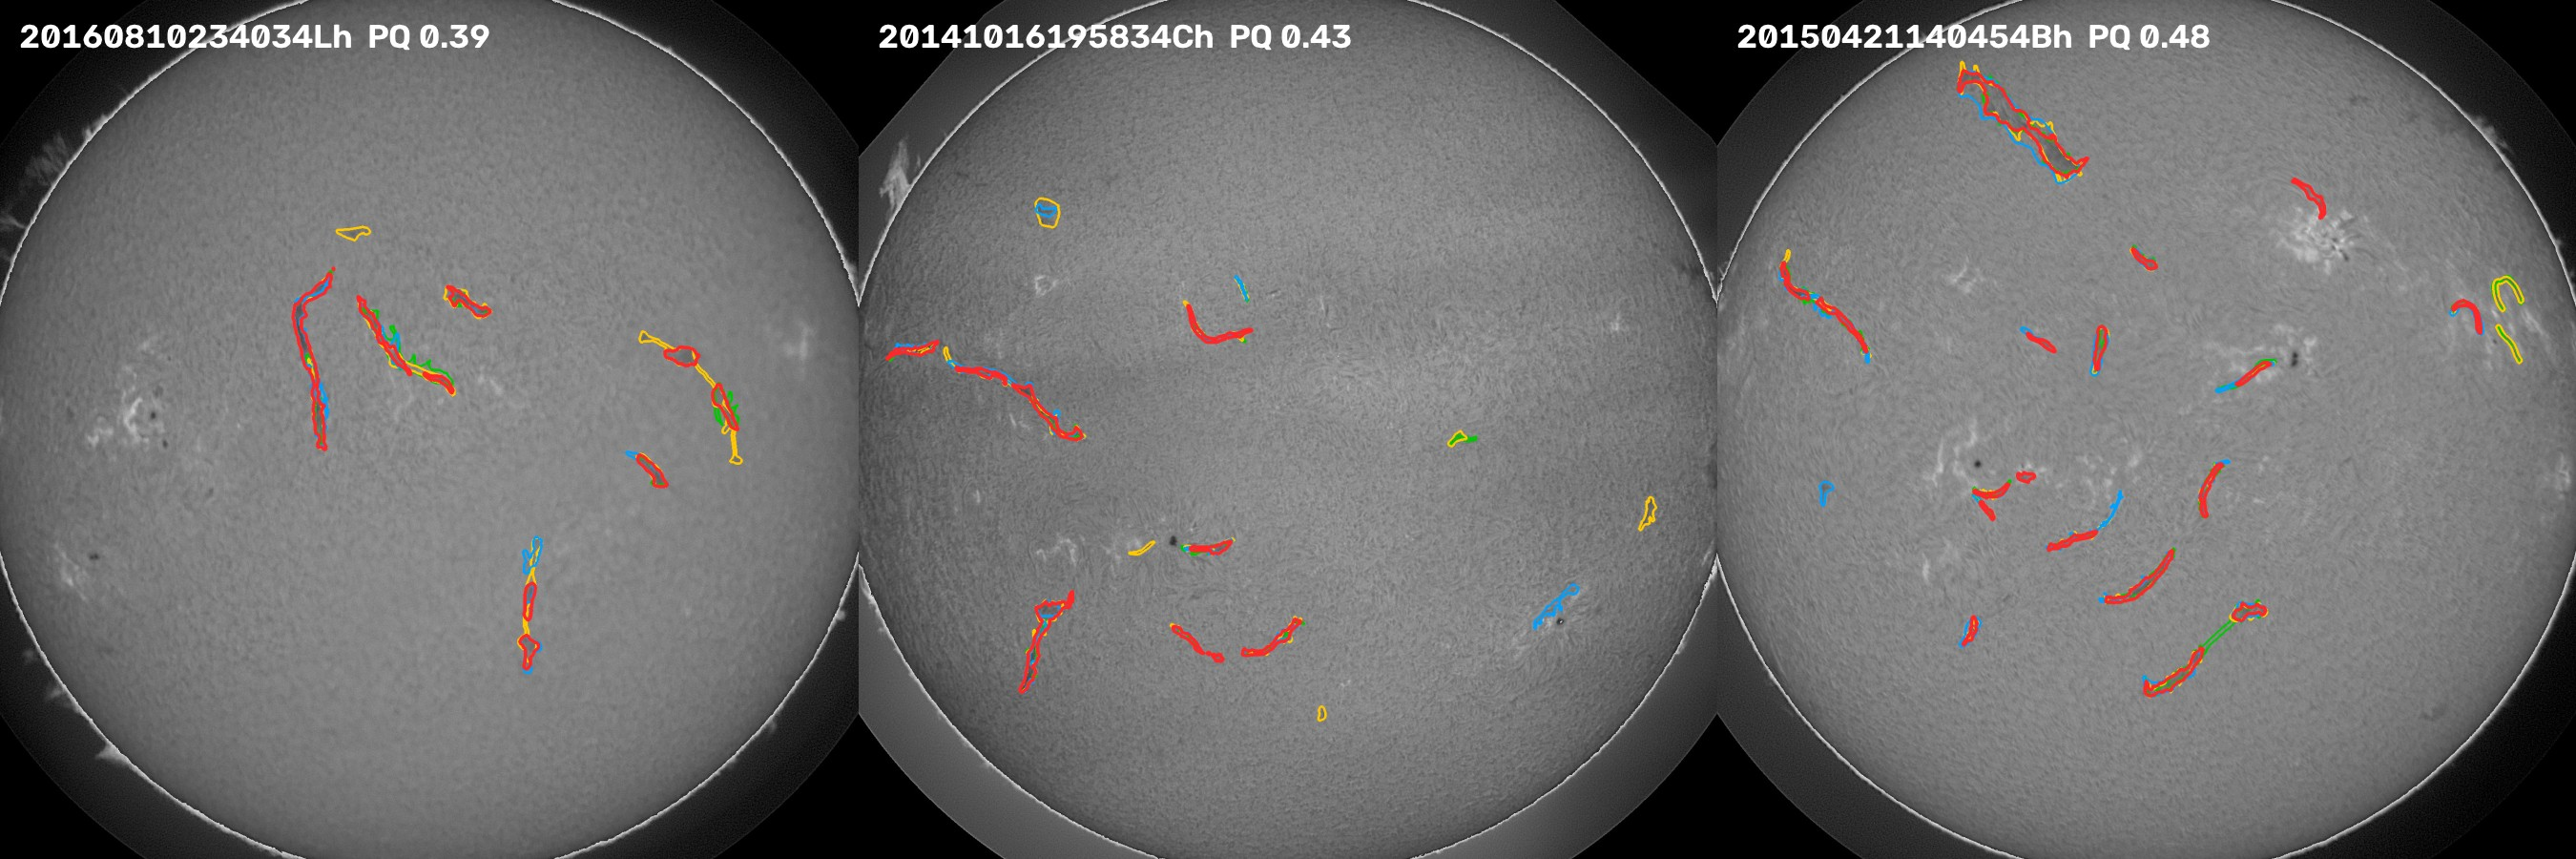
\includegraphics[width=\textwidth]{qualitative_final.jpg}
\caption{Out-of-fold predictions of the final pipeline (red) on three validation images with three annotators (green, yellow, blue), at the 50th, 75th and 90th percentile of image PQ among images with at least five filaments per annotator. Many misses are filaments marked by one annotator only.}
\label{fig:qual}
\end{figure*}


% ==================================== %
%              EVALUATION              %
% ==================================== %
\section{Evaluation}\label{sec:evaluation}

\subsection{Main results}
Table~\ref{tab:main} gives the main numbers. Uncertainty comes from two sources: the spread of PQ over the five folds, and a bootstrap that resamples whole images (all entries of an image together, 2{,}000 resamples) and recomputes the pooled PQ. The paired bootstrap of the difference to the previous pipeline resamples the same images for both. To put the numbers in scale, each annotator's masks are scored as predictions against every other annotator of the same image (296 images with two or three annotators).

\begin{table}[t]
\centering
\caption{Main results. OOF: out of fold, 707 images, 1{,}154 entries. Brackets: 95\% bootstrap interval over images.}
\label{tab:main}
\small\setlength{\tabcolsep}{3pt}
\begin{tabular}{@{}lccc@{}}
\toprule
 & PQ & SQ & RQ \\
\midrule
Final pipeline, OOF & \textbf{0.422} [0.412, 0.431] & 0.674 & 0.626 \\
\quad per fold, mean $\pm$ s.d. & 0.422 $\pm$ 0.012 & & \\
\quad 296 multi-annotator images & 0.423 & 0.671 & 0.630 \\
Annotator vs.\ annotator (same 296) & 0.340 & 0.634 & 0.536 \\
\midrule
1024~px, 2 views, hand rule, OOF & 0.409 [0.399, 0.418] & 0.666 & 0.614 \\
\quad + 4 views & 0.412 & 0.667 & 0.617 \\
\quad + component scorer & 0.417 & 0.668 & 0.624 \\
1536~px, 4 views, hand rule & 0.417 & 0.671 & 0.621 \\
Gain over 1024~px rule (paired) & +0.013 [0.008, 0.018] & & \\
\midrule
Public leaderboard, final pipeline & 0.35 & -- & -- \\
Public leaderboard, 1024~px rule & 0.35 & -- & -- \\
\bottomrule
\end{tabular}
\end{table}

The final pipeline improves on the previous one on all five folds (per fold: +0.017, +0.007, +0.013, +0.012, +0.018), and the paired bootstrap interval of the gain excludes zero. Its components contribute unequally: tuned per fold, 1536~px beats 1024~px on four of five folds (+0.009, $-0.002$, +0.009, +0.005, +0.007), and 2048~px matches 1536~px on the two folds tried. The scorer beats the submitted hand rule (confidence $\geq 0.8$) on every fold, by 0.002--0.009, but the best pooled hand rule (confidence $\geq 0.85$, PQ 0.420) by only 0.002. The two leaderboard scores are equal at the two decimals shown: scaled to the 90 or so public images, the bootstrap interval of a single pipeline is about $\pm$0.027, twice the gain. Local OOF ran 0.06--0.07 above the public leaderboard for every submission.

Fig.~\ref{fig:dist} shows the three evaluation plots requested by the organisers on the OOF predictions. Over GT/prediction pairs with IoU~$>0$, the mean IoU is 0.573 and the mean Dice 0.707 (0.553 and 0.688 for the 1024~px rule pipeline). 3.4\% of predicted filaments overlap more than one annotation (merges) and 3.7\% of annotations overlap more than one prediction (splits); 11.7\% of predictions overlap no annotation of their entry and 23.3\% of annotations overlap no prediction. Compared with the hand rule, the scorer removes a quarter of the false positives at the cost of more missed annotations, mostly filaments few annotators agree on. Fig.~\ref{fig:qual} shows typical images.

\begin{figure}[t]
\centering
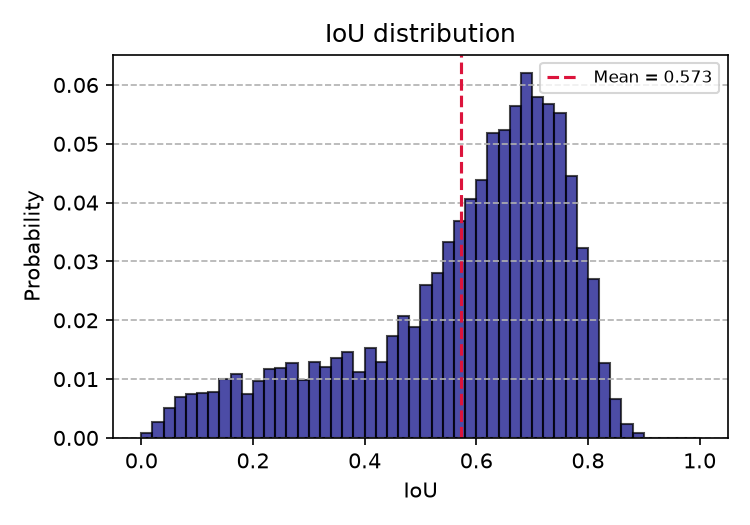
\includegraphics[width=0.49\linewidth]{oof1536_iou.png}\hfill
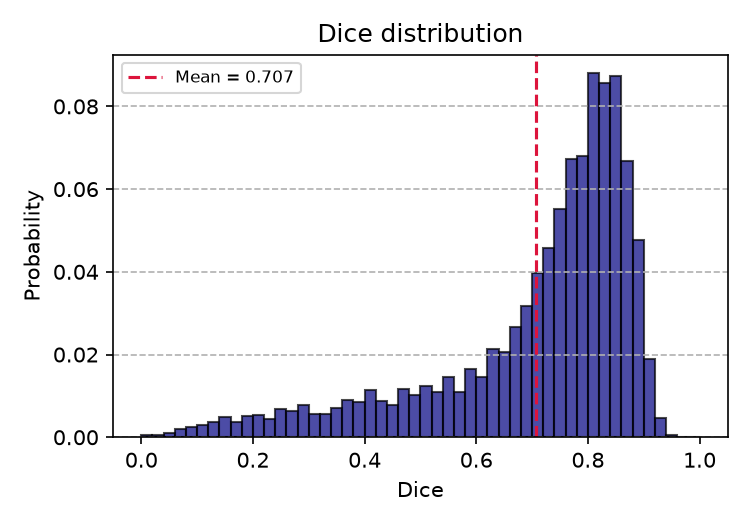
\includegraphics[width=0.49\linewidth]{oof1536_dice.png}\\[2pt]
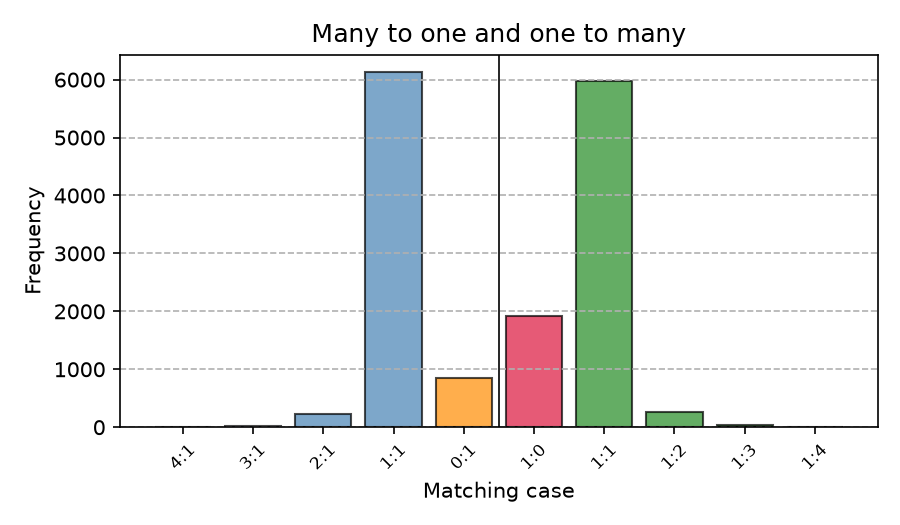
\includegraphics[width=0.9\linewidth]{oof1536_m2n.png}
\caption{Out-of-fold IoU and Dice distributions over GT/prediction pairs with IoU $>0$, and the one-to-many / many-to-one counts (left: number of GT linked to each prediction; right: number of predictions linked to each GT).}
\label{fig:dist}
\end{figure}

\subsection{What did not help}
Table~\ref{tab:abl} lists the variants we tried, each with its own tuned post-processing. A Mask R-CNN~\cite{maskrcnn} detector learns grouping explicitly, but its masks are coarser (SQ 0.642 vs.\ 0.657 for a U-Net trained for a similar number of epochs); adding its extra instances, or a per-filament crop refiner at native resolution following Reche \& Cid~\cite{reche2026}, changes PQ by less than 0.002 on the fully trained U-Net. A ResNet-50 encoder, an input divided by its own radial brightness profile (limb-darkening correction) and a Lov\'asz hinge loss~\cite{lovasz} match or underperform the baseline; with the corrected input the best threshold moves from 0.45 to 0.65, so the network becomes more confident but not more accurate. Averaging two equal-strength models with different encoders gives the PQ of the better one, and the 5-fold average gives the same leaderboard score as one model: the models share their errors because the errors come from the annotators, so the submission is one network.

\begin{table}[t]
\centering
\caption{Variants (fold 0, 142 images, tuned PQ) and post-processing rules (5-fold OOF, 707 images).}
\label{tab:abl}
\small
\begin{tabular}{@{}p{0.70\linewidth}r@{}}
\toprule
Variant (fold 0) & PQ \\
\midrule
U-Net ResNet-34, 40 epochs (baseline) & \textbf{0.416} \\
\quad 10 / 20 epochs & 0.389 / 0.396 \\
\quad + crop refiner at native resolution & 0.413 \\
\quad + Mask R-CNN instances not covered & 0.417 \\
Mask R-CNN alone (disjoint masks) & 0.377 \\
ResNet-50 encoder & 0.414 \\
Limb-darkening-corrected input & 0.411 \\
BCE + Lov\'asz hinge & 0.390 \\
Average of ResNet-34 and ResNet-50 & 0.416 \\
8 dihedral views (4 flips: 0.419) & 0.419 \\
2048~px, folds 0 / 3 (1536~px: 0.403 / 0.387) & 0.404 / 0.388 \\
\midrule
Post-processing rule (OOF, 1024~px) & PQ \\
\midrule
Submission setting (confidence $\geq 0.8$) & 0.409 \\
Confidence $\geq 0.85$ & 0.411 \\
No closing, no confidence or limb filter & 0.398 \\
Size-dependent confidence threshold & 0.411 \\
Hysteresis (seed and grow thresholds) & 0.409 \\
Masks dilated / eroded by 1~px & 0.381 / 0.399 \\
70-degree limb cut-off & no change \\
\bottomrule
\end{tabular}
\end{table}

\subsection{Where the remaining PQ is lost}\label{sec:loss}
\emph{Near misses.} Of the 3{,}174 OOF false negatives, 45\% overlap no prediction, 18\% overlap one at IoU $<0.3$ and 37\% at IoU 0.3--0.5. Among the near misses the prediction is smaller than the GT in 46\% of cases and larger in 34\%; only 17\% are merges with another filament and 16\% splits. Dilating or eroding every mask by one pixel costs 0.01--0.03 PQ, because filaments are only a few pixels wide: the extent errors are per instance, not a bias a rule could correct.
\emph{Small filaments.} Recall falls to 0.36 below 500~px. Annotators rarely agree on them: the share of other annotators marking the same filament (IoU $>0.5$) is 0.28 below 300~px and about 0.60 above 1{,}000~px.
\emph{When a doubtful prediction pays.} A prediction matching $k$ of $n$ annotators raises PQ only if $k/n > \mathrm{PQ}/(2\,\mathrm{SQ}) \approx 0.31$. A filament marked by one annotator of three is break-even, which is why lowering the area or confidence thresholds never helped; 28\% of our false positives match another annotator's filament on the same image.

\subsection{Strengths, weaknesses and possible improvements}
\emph{Strengths.} One network and a small tree model, no external data, 4.5~s per image, and a submission reproduced byte for byte by the notebook. Out of fold it exceeds a single annotator on both boundary quality (SQ) and detection (RQ): trained on the consensus, it predicts the filaments most annotators agree on. The scorer optimises the metric directly and needs no hand-tuned thresholds.
\emph{Weaknesses.} Missed annotations are now the largest error (23\% of annotations overlap no prediction), mostly small filaments and filaments marked by one annotator; extent errors of one or two pixels on thin filaments cost SQ; and the gain over the previous pipeline is small relative to the leaderboard's resolution.
\emph{Improvements.} Since most of the remaining loss is disagreement between annotators, further gains should come from modelling the annotators (for example a head per annotator, or predicting each annotator's style) rather than from a stronger segmenter; a second-stage scorer could also be given image context beyond the two image-level features.


% ==================================== %
%            ACKNOWLEDGMENT            %
% ==================================== %
\section{Acknowledgment}\label{sec:acknowledgment}
    % Do not change
    The organization of the Filament Segmentation Challenge 2026 is partially supported by the U.S. National Science Foundation (NSF) under Grant No. 2209912 and 2433781, directorate for Computer and Information Science and Engineering (CSE), and Office of Advanced Cyberinfrastructure (OAC), and Grant No. 2511630, AST Division Of Astronomical Sciences and MPS Directorate for Mathematical and Physical Sciences.

    The Filament Segmentation Challenge 2026 is sponsored by the U.S. National Science Foundation (NSF) National Solar Observatory (NSO).

    This work utilizes GONG data obtained by the NSO Integrated Synoptic Program, managed by the National Solar Observatory, which is operated by the Association of Universities for Research in Astronomy (AURA), Inc. under a cooperative agreement with the National Science Foundation and with contribution from the National Oceanic and Atmospheric Administration. The GONG network of instruments is hosted by the Big Bear Solar Observatory, High Altitude Observatory, Learmonth Solar Observatory, Udaipur Solar Observatory, Instituto de Astrofísica de Canarias, and Cerro Tololo Interamerican Observatory.

\bibliographystyle{ACM-Reference-Format}
\bibliography{main}

\end{document}
